% ************ Chapter 4 ************
\chapter{Projeção do Sistema de Informação} 
\label{cap:4}
Levantados os requisitos do projeto, iniciou-se projeção do sistema. Este foi um processo que envolveu desde planeamento de trabalho a ser realizado, ao design da aplicação.

\section{Planeamento do projeto}
A primeira semana do período do estágio foram destinadas ao levantamento de requisitos. Foi ainda durante esta semana que ocorreu o redesign da base de dados.
As semanas 2 e 3 foram destinadas ao estudo dos \textit{frameworks} a utilizar, do sistema de gestão de base de dados e do ambiente da empresa.
Conforme indicado nos requisitos do projeto, o desenvolvimento do sistema de informação teria de ser dividido em duas fases. A data para a conclusão da primeira fase foi fixada no inicio da sexta semana, dando-se logo incio à fase dois.

\section{Design da nova base de dados}
A base de dados a ser utilizada neste projeto teve como ponto de partida aquela que já era utilizada pela aplicação antiga. De modo a tornar a estrutura o mais adequada possível, numa da reuniões, foi solicitado à administração que descrevesse em detalhe o fluxo de informação da estrutura até à data implementada. Após a reunião seguiu-se um estudo para encontrar formas de otimizar a estrutura da base de dados, não apenas na questão da normalização da estrutura mas também de forma a tornar o trabalho futuro mais simples procurando meios de otimizar o fluxo da informação. Após o estudo foi entregue de uma proposta da nova estrutura. Esta foi chumbada numa fase inicial porque, como resultado da normalização, foi criada uma tabela destinada a armazenar os cemitérios com os quais a empresa tem parceria, uma segunda tabela onde ficaram registadas as empresas a quem a Natural Life compra o materia-prima e uma terceira tabela responsável por agregar os registos das primeiras duas de modo a estabelecer as relações com a restantes tabelas do sistema. A reposta da administração foi que preferia que existisse apenas uma única tabela, que agregasse os campos das três referidas anteriormente, com um campo extra para distinguir o tipo de registo. Apesar de compreenderem qual era o intuito da mudança sugerida, esta iria tornar mais difícil a adaptação de ficheiros Excel e PowerBi já existentes. A mudança pedida foi efetuada e a administração aceitou as restantes alterações sugeridas. Dentre dela destaca-se a tabela "Entidades" criada para armazenar as informações de identificação (nome, morada, código postal e nif) dos pontos de recolha e clientes. Esta alteração permitiu não só reunir num único local a lista de entidades com as quais a Natural Life interage, eliminado eventuais incoerências de informação a respeito do numero de identificação fiscal, por exemplo.
O processo de reforma da base de dados manteve-se então congelado até à sétima semana, na qual se criou a tabela "completar\_recolha", conforme descrito no capítulo anterior. No final de todo este processo a estrutura final da base de dados, aprovada pela administração, é a descrita na figura \ref{fig:db_model}.

\begin{figure}[htbp] 
	\begin{center}
		% Requires \usepackage{graphicx}
		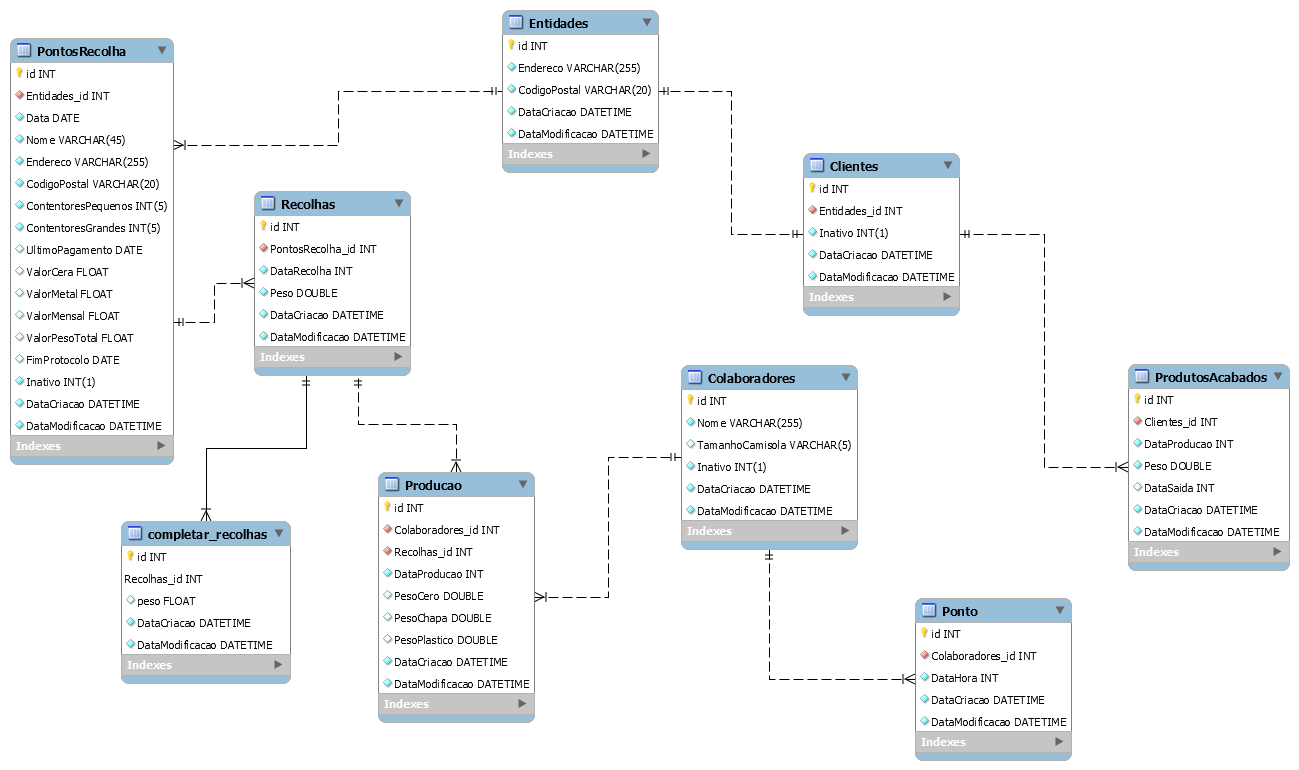
\includegraphics[width=\textwidth,keepaspectratio]{figuras/DB_Model/new.png}
		\caption{Estrutura final da base de dados}
		\label{fig:db_model} 
	\end{center}
\end{figure}

Finalizado este processo, iniciou-se o processo de design da aplicação.

\section{Aplicação}
Respondendo aos requisitos definidos no Capitulo \ref{cap:3}, a aplicação a ser desenvolvida seria uma aplicação web construída em PHP, com o framwork laravel, e JavaScript segundo o padrão do modelo MVC. O modelo MVC, representado na figura \ref{fig:mvc}, descreve a forma como uma aplicação deve ser construída separando-a em três camadas distintas: Model View e Controller. Esta separação server distinguir representações de informação internas dos modos como a informação é apresentada ao utilizador\cite{Wikipediad}.
Esta abstração em camadas é particularmente vantajosa no que toca a fazer reutilização de código, pois tendo em conta as regras do modelo cada classe tem apenas uma responsabilidade atribuída além de o projeto ter um baixo acoplamento entre si. Desta forma é muito fácil utilizar a mesma classe partes distas do projeto, facilitando a sua compreensão, manutenção e atualização.
Estas características do modelo servem ainda de resposta a outros requisitos do projeto como modularidade do projeto.
\begin{figure}[H] 
	\begin{center}
		% Requires \usepackage{graphicx}
		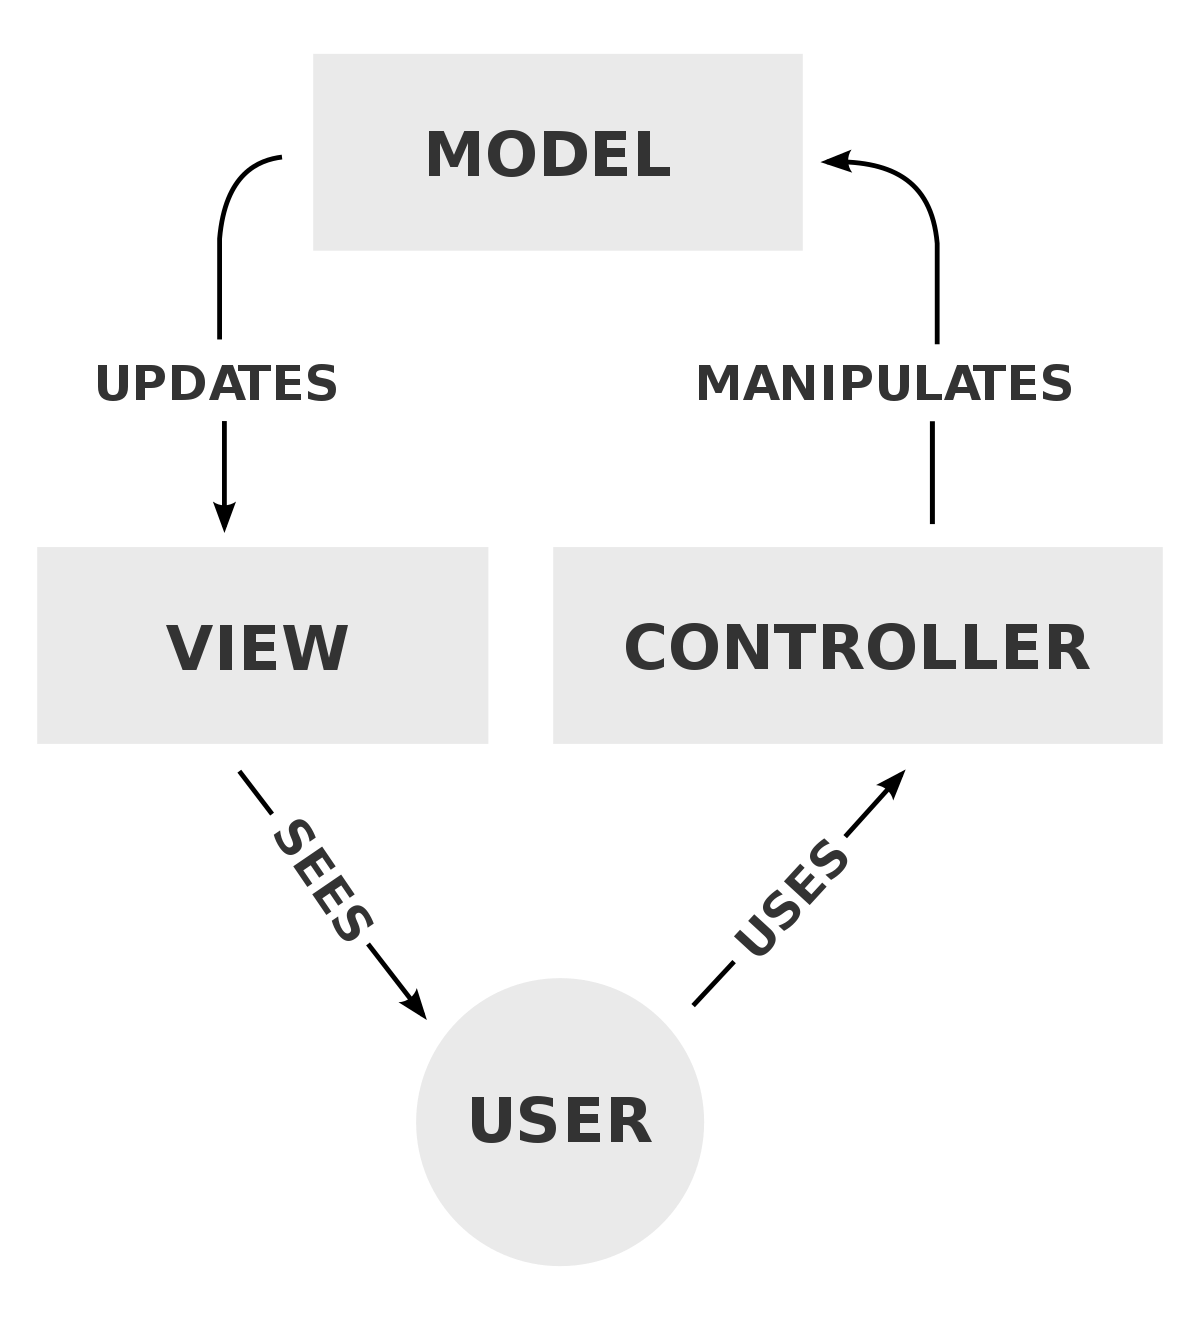
\includegraphics[width=0.30\textwidth,keepaspectratio]{figuras/mvc.png}
		\caption{Diagrama do modelo MVC}
		\label{fig:mvc} 
	\end{center}
\end{figure}

\noindent 
Ainda respondendo aos requisitos deveria existir duas áreas distintas dentro da aplicação destinada aos colaboradores na fábrica e à administração.
Estas suas sub-aplicações foram designadas de Aplicação Fábrica, acessível aos colaboradores da empresa e responsável pelos registos de informação na base de dados, e a Aplicação Painel, protegida por um sistema de autenticação na qual seria possível manipular toda a informação registada.
Para fazer esta separação, os endereços dentro da aplicação foram divididos em dois grupos distintos. Em primeiro lugar as páginas associadas à Aplicação de Fábrica estavam sob o endereço /Fabrica:

\begin{center}
\url{http://<ip.do.servidor>/Fabrica/<Nome_da_página_solicitada>}
\end{center}

\noindent 
Enquanto as páginas relacionadas com a Aplicação Painel estavam sob o endereço /Painel:

\begin{center}
	\url{http://<ip.do.servidor>/Painel/<Nome_da_página_solicitada>}
\end{center}

\noindent 
A única exceção a esta regra está no diretório raiz do sistema, que direciona para a página index da Aplicação de Fábrica.\\
Esta organização em nada muda a estrutura de ficheiros do projeto. O framework laravel, trás consigo um recurso de rotas, que permite facilmente que este tipo de regras seja incluída no projeto sem ter necessariamente que fazer modificações à árvore de diretórios da aplicação. Desta forma, manteve-se uma estrutura dos ficheiros da aplicação coesa, mantendo cada tipo de ficheiro na sua pasta definida e manter regras de padronização dos endereços da aplicação.

\section{Casos de uso do sistema}
Definidos todos os detalhes supracitados, é possível dar inicio à definição de cada um dos casos de uso do projeto. Esta definição serve como guia de desenvolvimento, mantendo as informações necessárias para se conhecer o comportamento esperado de cada um dos casos de uso do sistema final e é explicada nas próximas páginas.
\newpage

% Aplicação Fábrica
\subsection{Aplicação Fábrica: Menu Inicial}
\subsubsection*{Descrição do caso de uso}
No menu, espera-se que este seja muito simples e intuitivo. Deve conter botões que indiquem de forma inequívoca qual a qual funcionalidade dão acesso. As cores das opções já existentes na aplicação construida no Microsoft Access deverão ter cores similares.\\
Na primeira fase do projeto este menu deve apenas contemplar as opções existentes na aplicação anterior, tal como descrito na figura \ref{fig:di_fabrica_menu} a.\\
No final da segunda fase, espera-se que o menu inicial apenas acrescente dois botões no final, conforme demonstrado na figura \ref{fig:di_fabrica_menu} b

\begin{figure}[H]
	\centering
	
	\begin{subfigure}[t]{0.45\linewidth}
		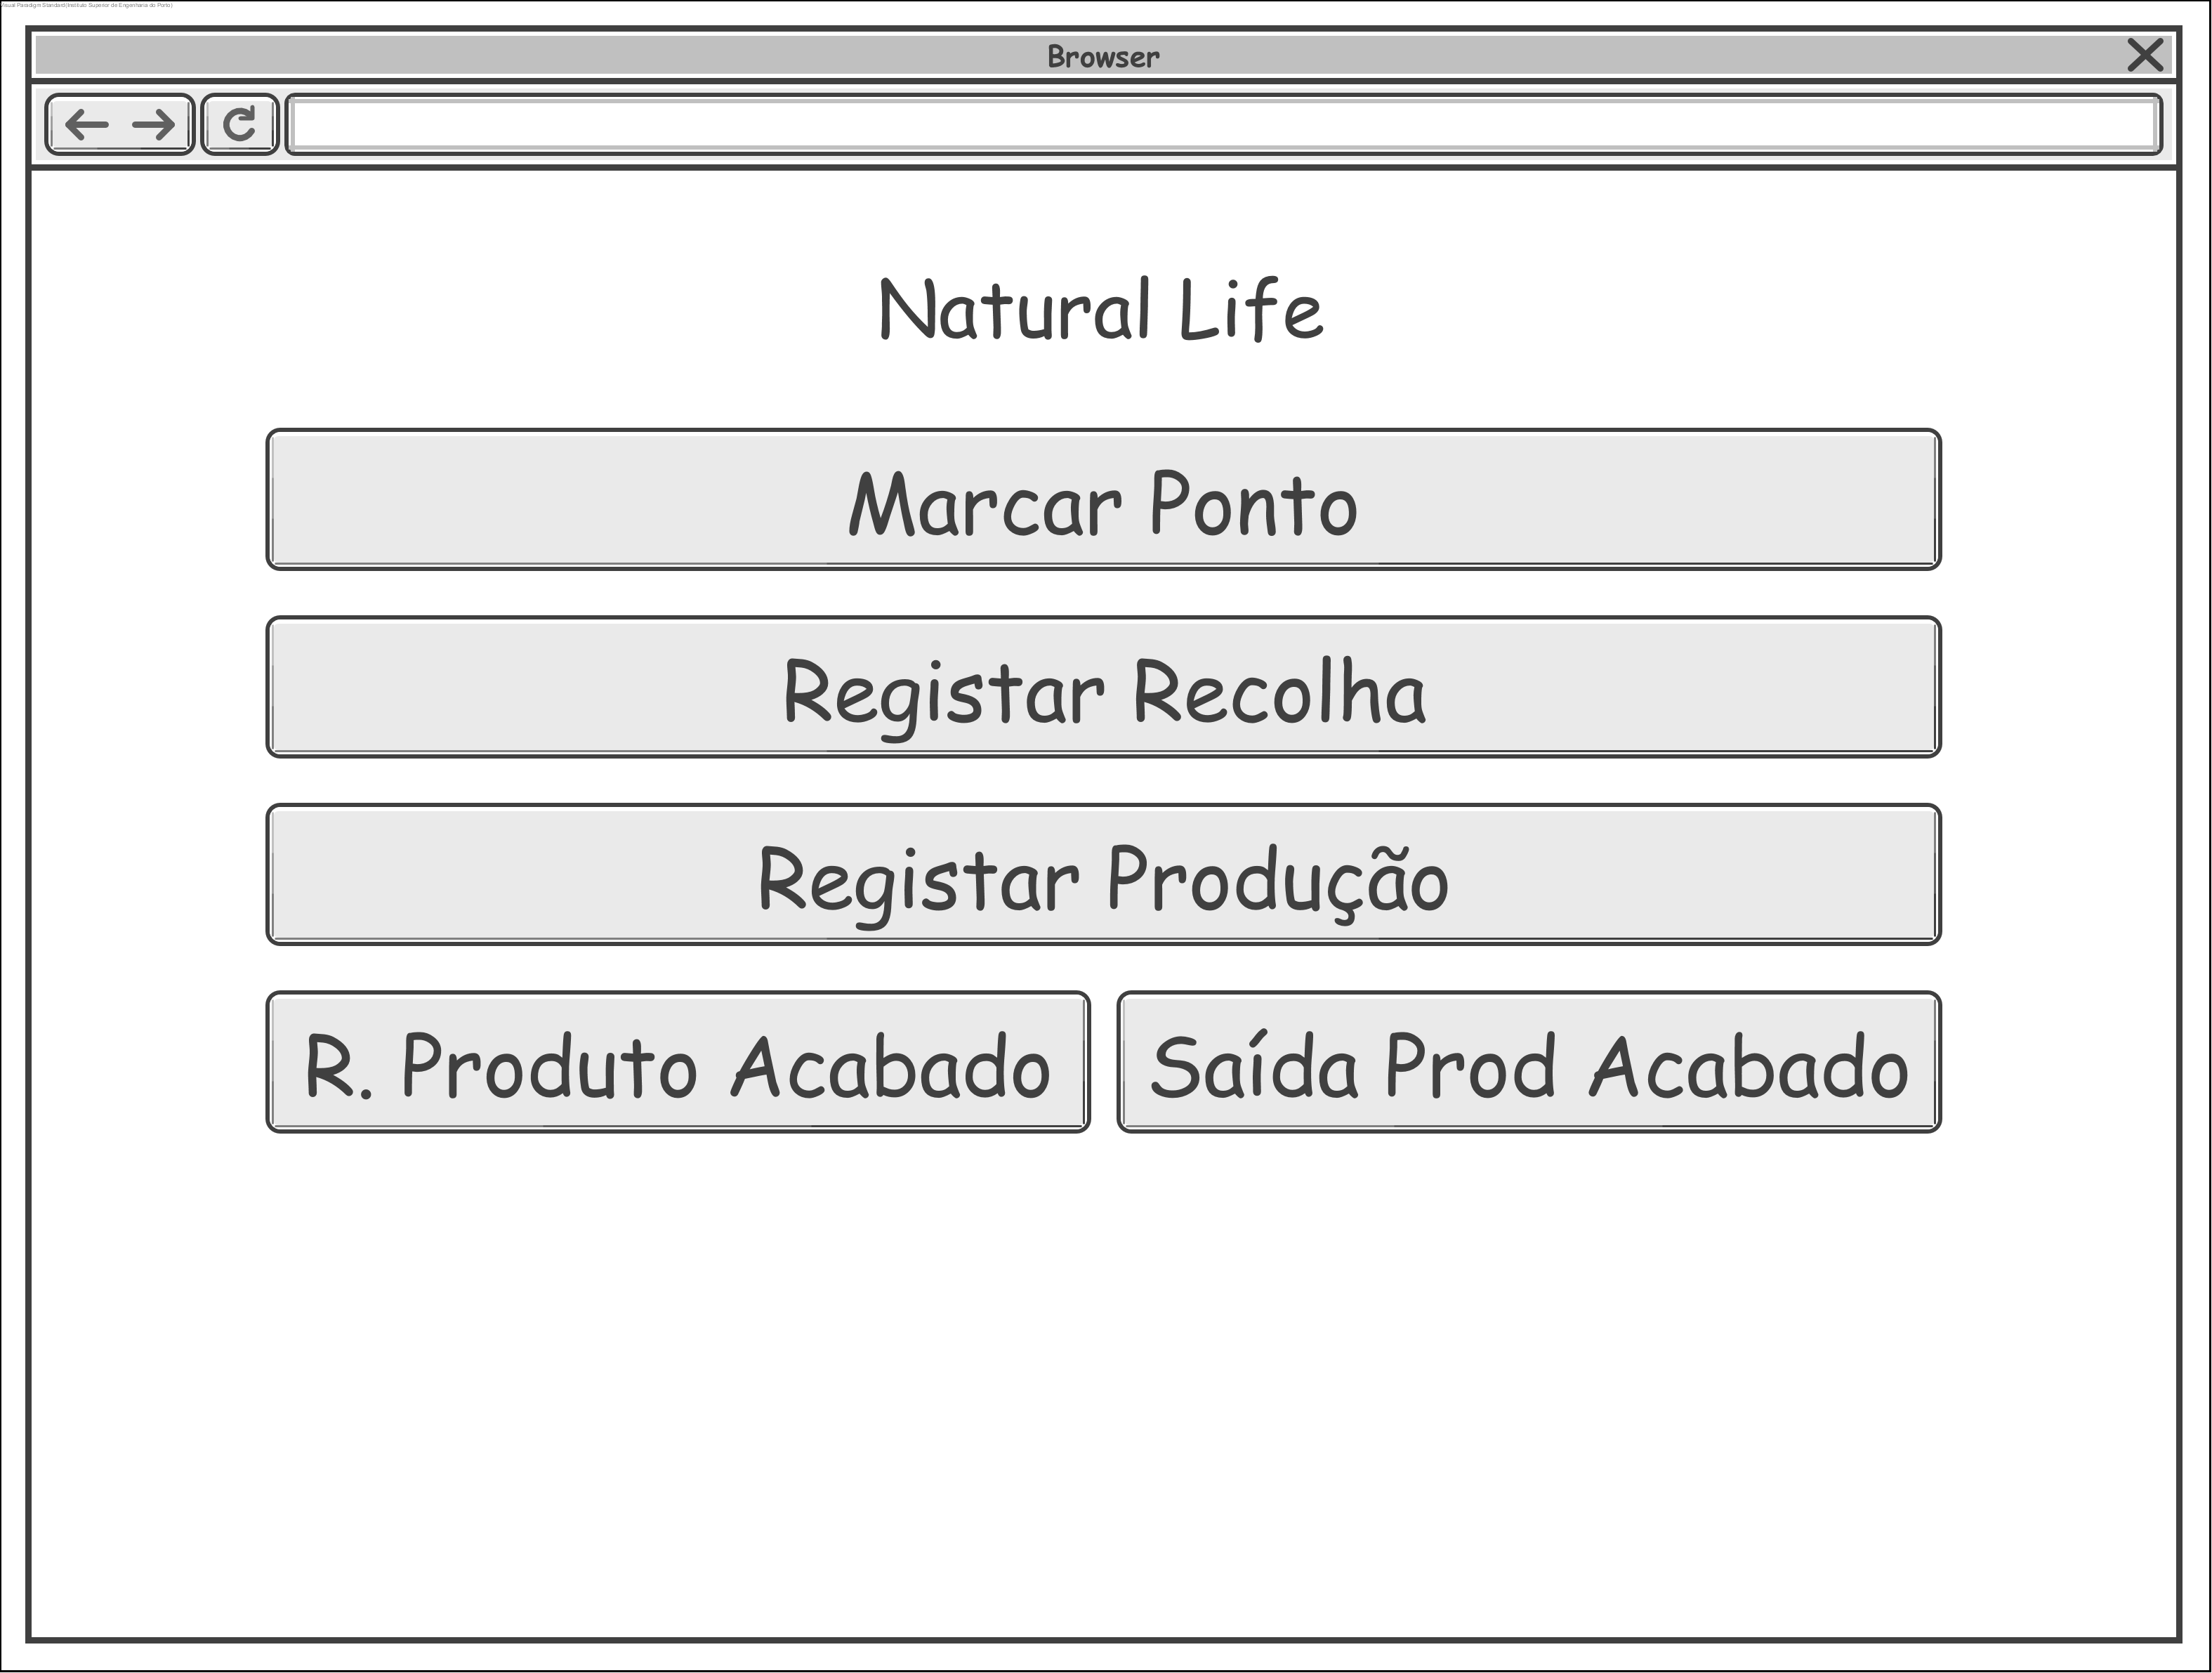
\includegraphics[width=\linewidth]{figuras/Diagramas_vp/DI_Fabrica_0-Menu_Inicial_-1a_Fase.png}
		\label{fig:di_fabrica_menu_1}
		\caption{Após concluir primeira fase}
	\end{subfigure}
	\begin{subfigure}[t]{0.45\linewidth}
		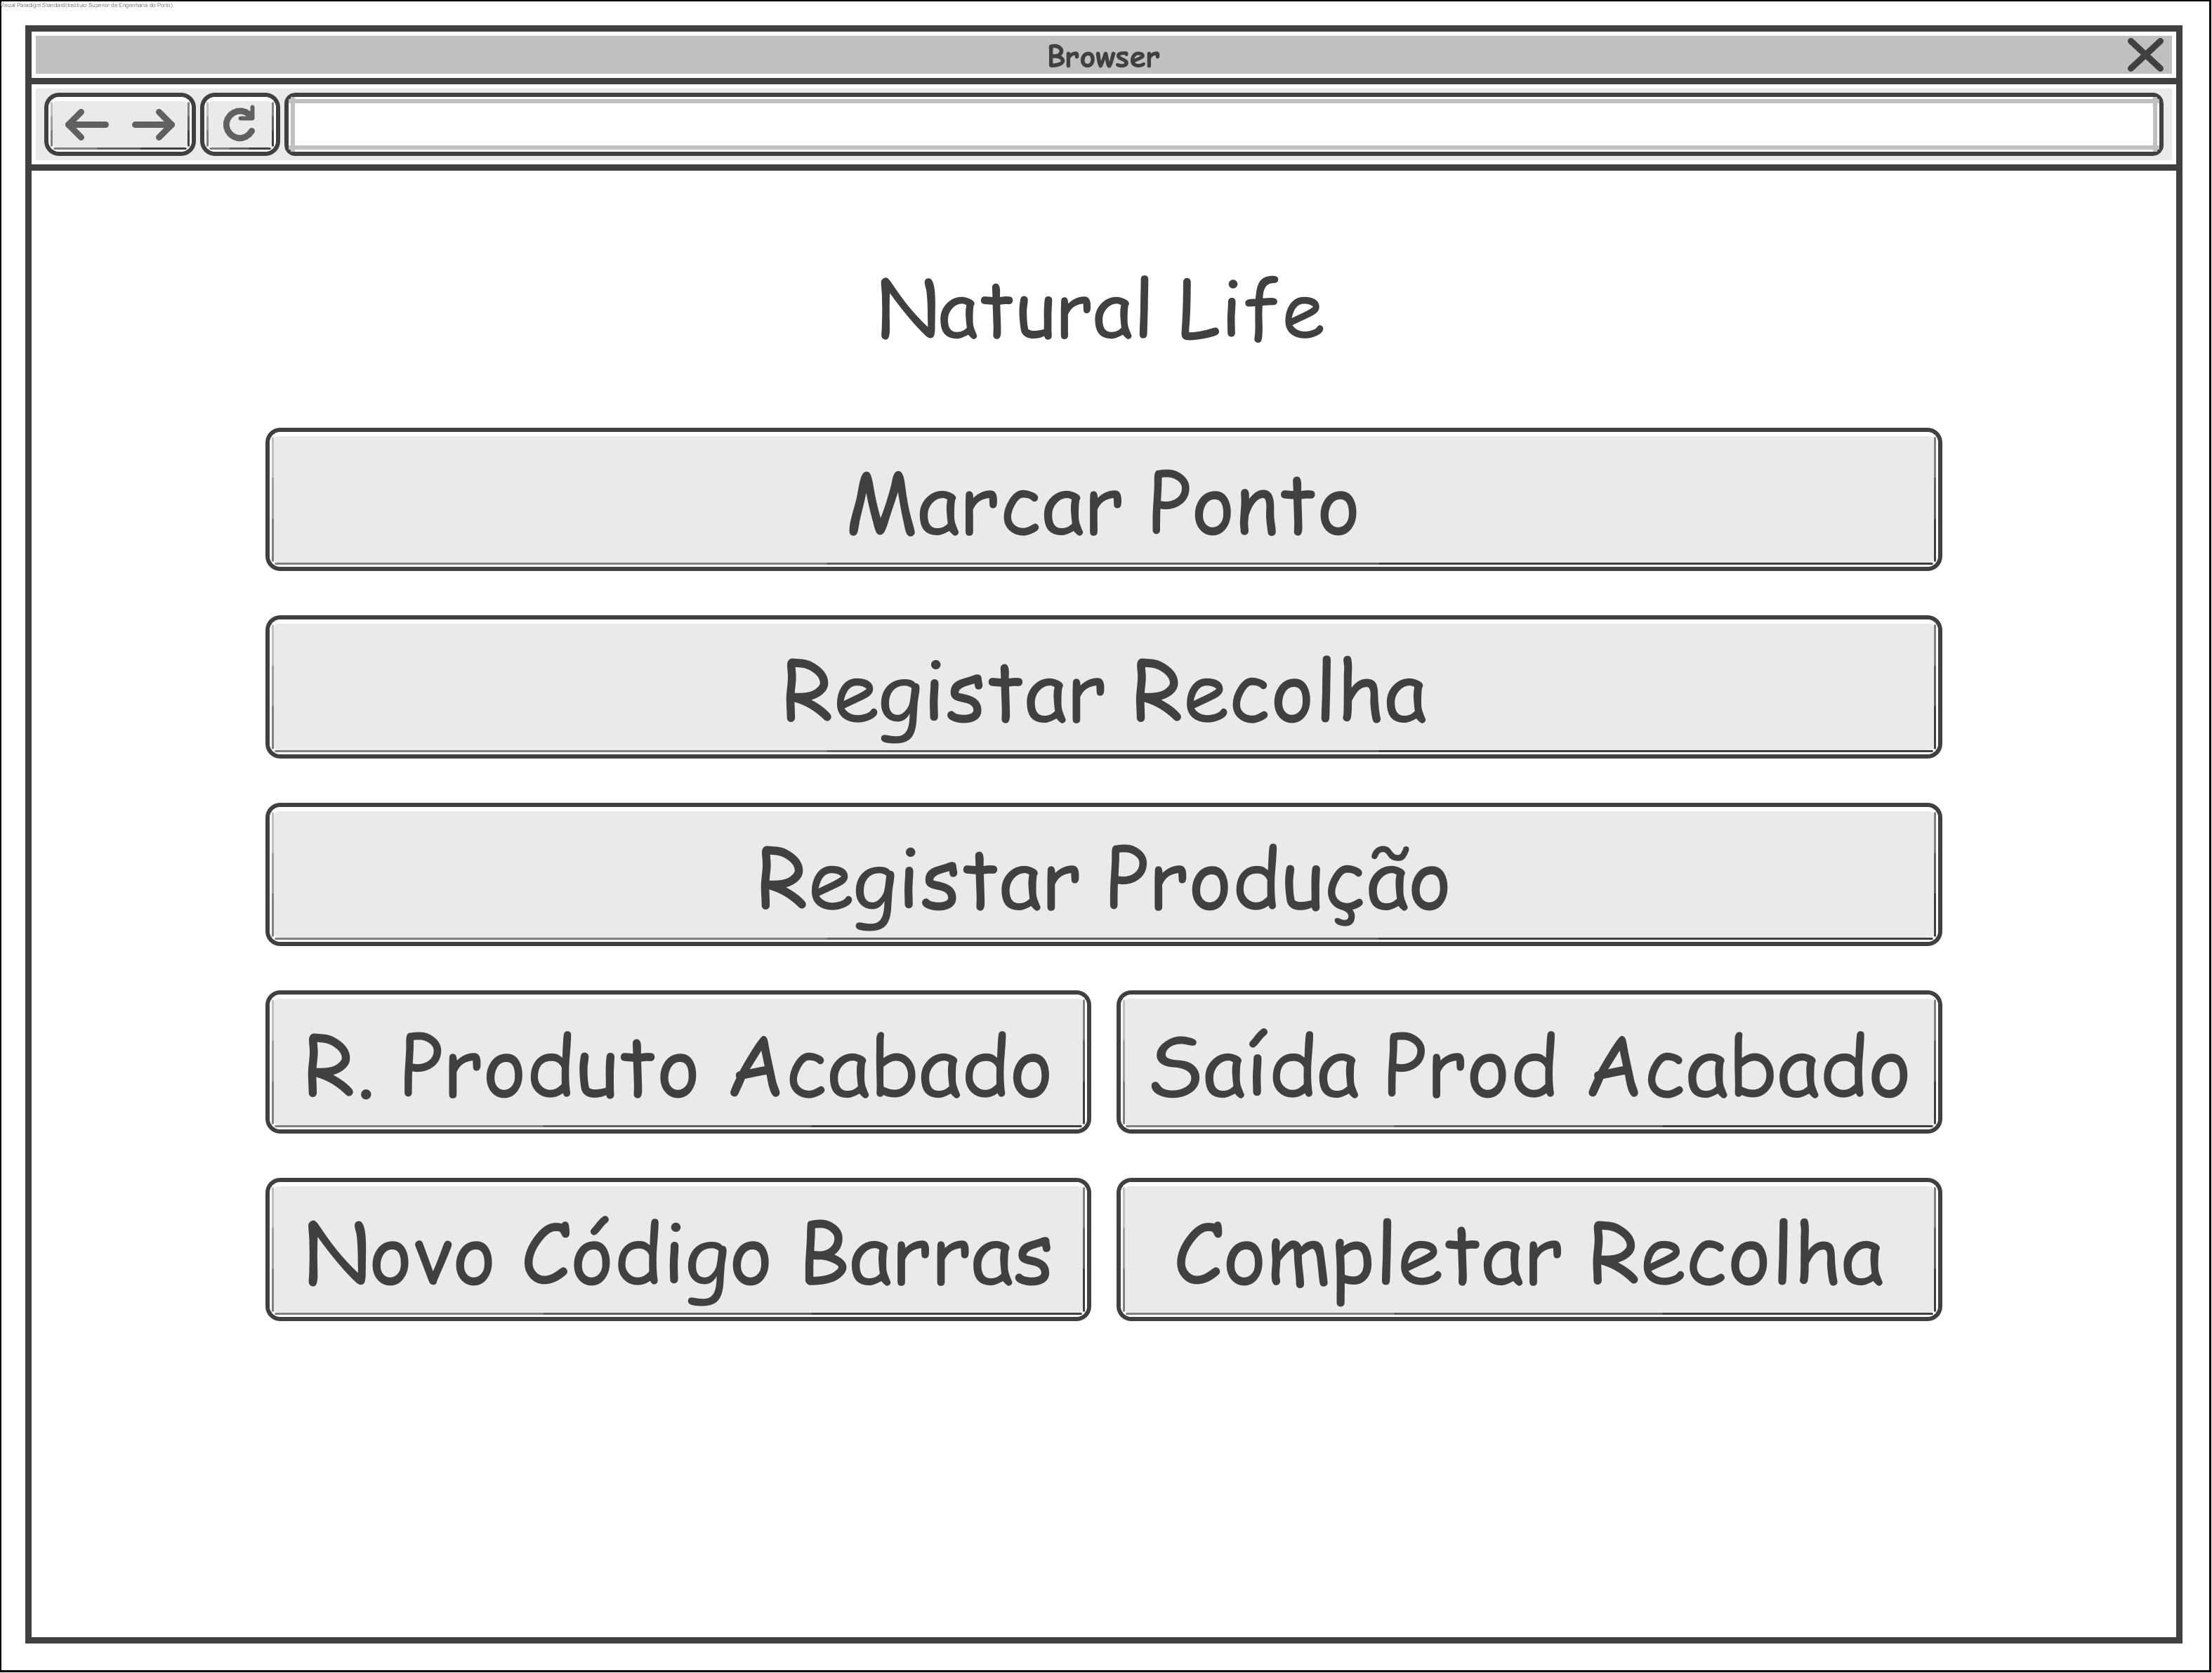
\includegraphics[width=\linewidth]{figuras/Diagramas_vp/DI_Fabrica_0-Menu_Inicial_-2a_Fase.png}
		\label{fig:di_fabrica_menu_2}
		\caption{Após concluir segunda fase}
	\end{subfigure}
	
	\caption{Modelo do menu}
	\label{fig:di_fabrica_menu}
\end{figure}
\newpage
\subsection{Aplicação Fábrica: Registo de Ponto}
\subsubsection*{Descrição do caso de uso}
No registo do ponto, espera-se que utilizador entre na página e indique apenas o seu ID. A informação sobre a data e hora do registo deve ser automaticamente definida pelo sistema. 

\begin{figure}[H] 
	\begin{center}
		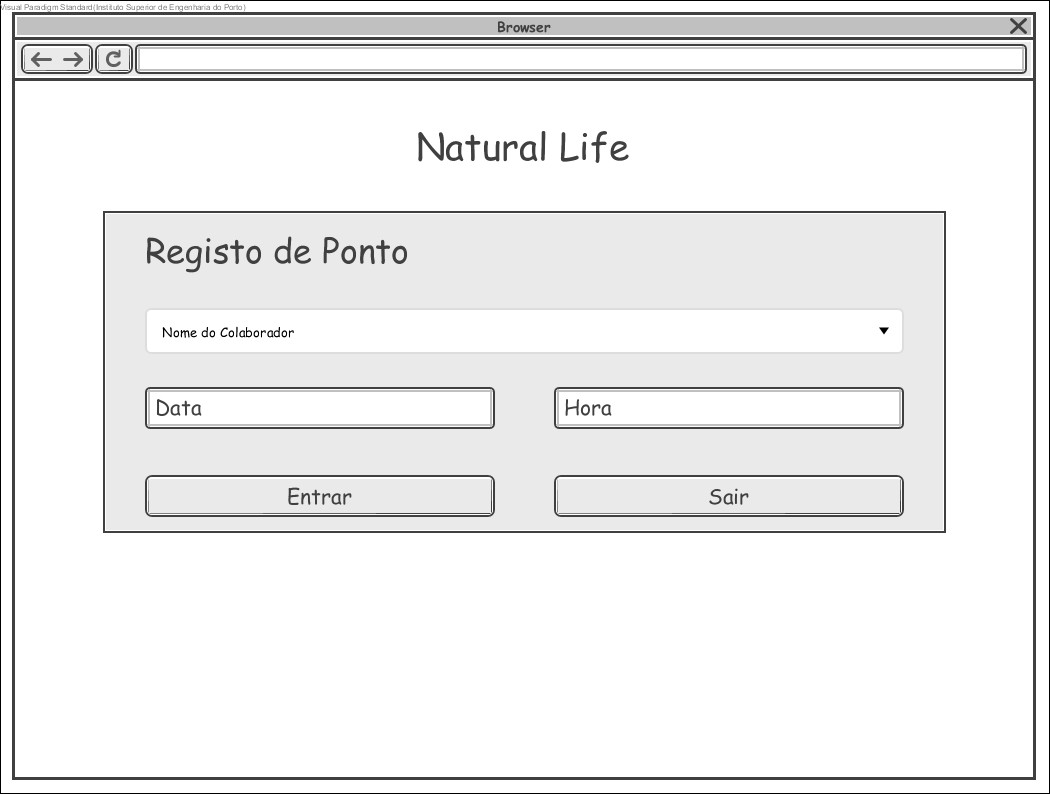
\includegraphics[width=0.60\textwidth,keepaspectratio]{figuras/Diagramas_vp/DI_Fabrica_1_Marcar_Ponto.jpg}
		\caption{Modelo do formulário do registo do ponto}
		\label{fig:di_ponto} 
	\end{center}
\end{figure}

\subsubsection*{Fluxo do caso de uso}
O caso de uso inicia-se com a abertura da página do registo de ponto. É apresentado o formulário com a data e hora previamente preenchidas. O utilizador tem de indicar o seu ID numa lista de dropdown. Após indicar o seu ID precisona o botão "Entrada" ou "Saída" conforme se esta a indicar o horario de entrada ou saída, respetivamente. Ambos os botões executam a submissão do formulário. Após o registo é apresentada uma mensagem ao utilizador


\begin{figure}[H] 
	\begin{center}
		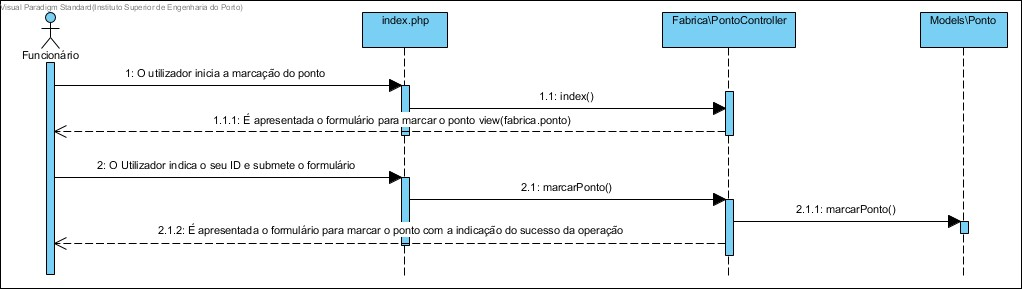
\includegraphics[width=\textwidth,keepaspectratio]{figuras/Diagramas_vp/SD_Fabrica_1_Marcar_Ponto.jpg}
		\caption{Diagrama de sequência marcar ponto}
		\label{fig:sd_ponto} 
	\end{center}
\end{figure}
\newpage
\subsection{Aplicação Fábrica - Registo de recolha}
\subsubsection*{Descrição do caso de uso}
No registo de recolha, espera-se que utilizador entre na página e indique o ID do ponto de recolha e o peso da recolha. A informação da data deve ser indicada automaticamente pelo sistema. A aparência da \textit{view} deste caso de utilização será semelhante ao demonstrado na figura \ref{fig:di_recolha}. 

\begin{figure}[H] 
	\begin{center}
		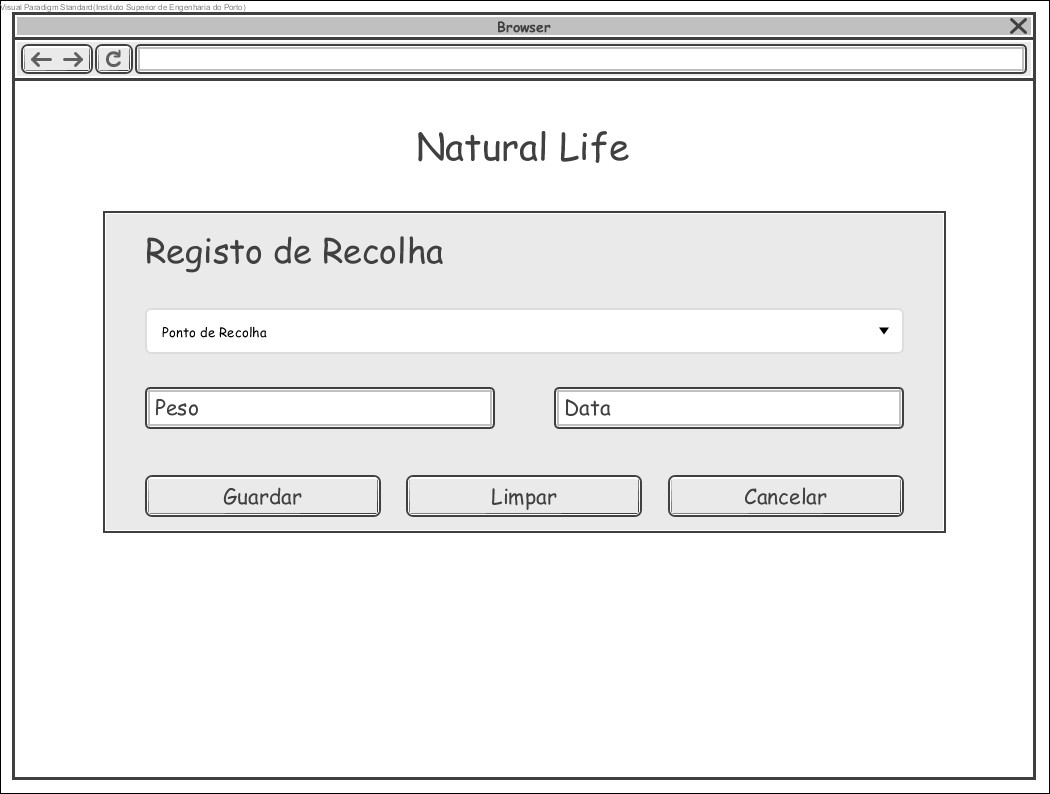
\includegraphics[width=0.60\textwidth,keepaspectratio]{figuras/Diagramas_vp/DI_Fabrica_2_Registo_de_Recolha.jpg}
		\caption{Modelo do formulário do registo de recolha}
		\label{fig:di_recolha} 
	\end{center}
\end{figure}

\subsubsection*{Fluxo do caso de utilização}
O caso de uso inicia-se com a abertura da página do registo de recolha. É apresentado o formulário com a data previamente preenchida. O utilizador tem de indicar o ID do ponto de recolha numa lista de \textit{dropdown} e o peso da recolha feita. Após indicar as informações solicitadas precisona o botão \textit{Guardar}. No final do registo é apresentada uma mensagem ao utilizador. Caso o registo seja feito com sucesso um novo separador é aberto com o código de barras para ser impresso, tal como demonstrado na figura \ref{fig:sd_recolha}.


\begin{figure}[H] 
	\begin{center}
		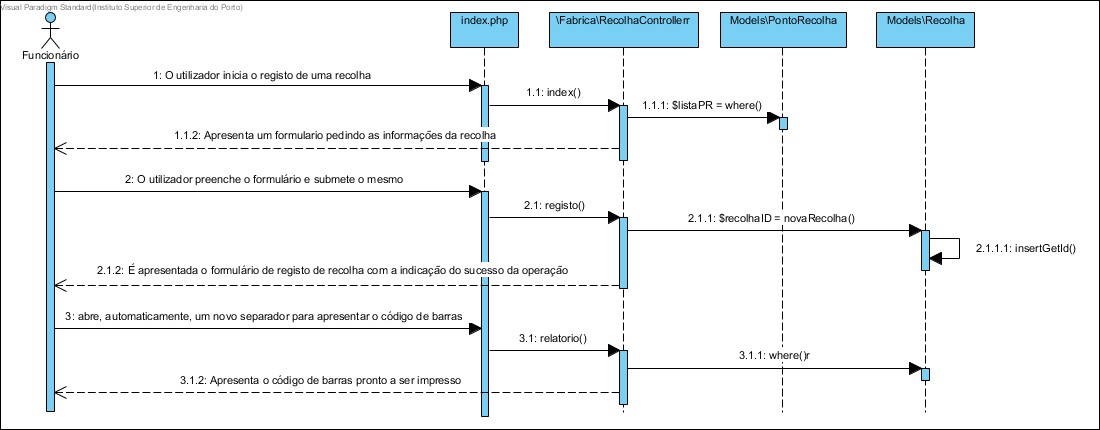
\includegraphics[width=\textwidth,keepaspectratio]{figuras/Diagramas_vp/SD_Fabrica_2_Registo_de_Recolhas.jpg}
		\caption{Diagrama de sequência registo de recolha}
		\label{fig:sd_recolha} 
	\end{center}
\end{figure}
\newpage
\subsection{Aplicação Fábrica: Produção}
\subsubsection*{Descrição do caso de uso}
No registo de produção, espera-se que utilizador entre na página e indique o código de barras da recolha, o peso de cera, metal e plástico e o seu ID. A informação da data de produção deve ser indicada automaticamente pelo sistema e a informação sobre a recolha (ponto de recolha e data da recolha) seja obtido, em background, após indicar o código de barras da recolha.

%\begin{figure}[H] 
%	\begin{center}
%		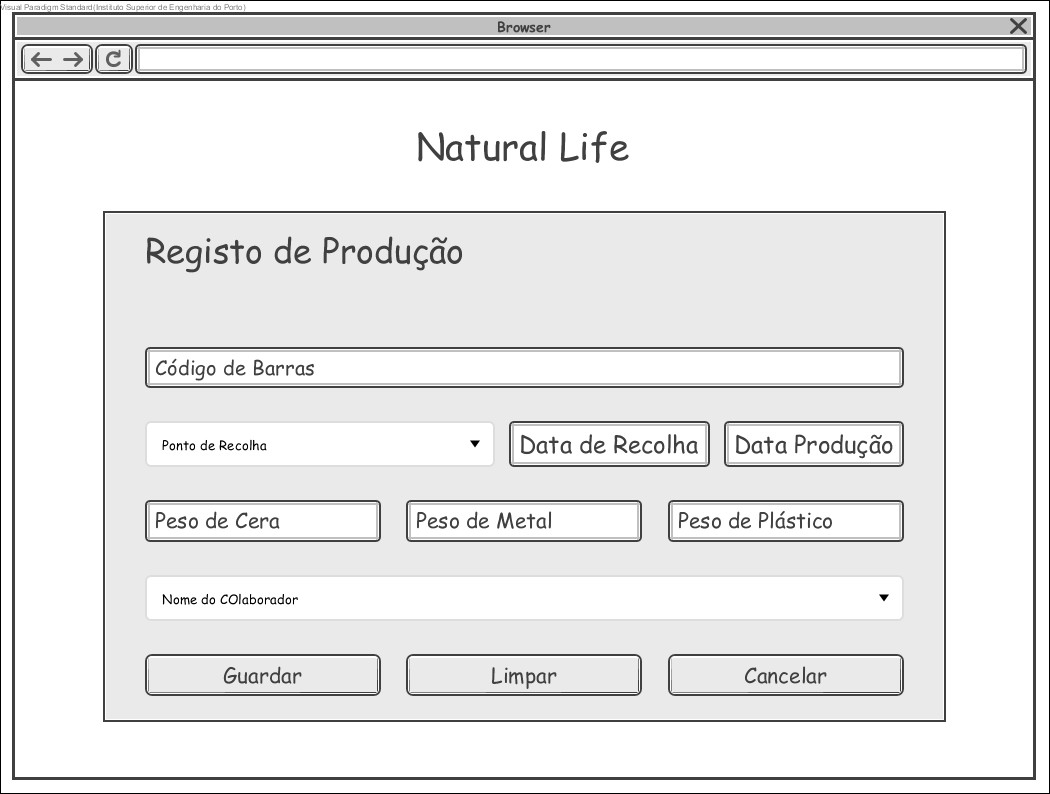
\includegraphics[width=0.60\textwidth,keepaspectratio]{figuras/Diagramas_vp/DI_Fabrica_3_Registo_de_Produção.jpg}
%		\caption{Modelo do formulário do registo de produção}
%		\label{fig:di_producao} 
%	\end{center}
%\end{figure}
\todo{falta os diagramas}

\subsubsection*{Fluxo do caso de uso}
O caso de uso inicia-se com a abertura da página do registo de produção. É apresentado o formulário com a data de produção previamente preenchida. O utilizador tem de indicar o código de barras da recolha, peso de cera, metal e plástico e o seu ID numa lista de dropdown. Quando o utilizador termina de indicar o código da recolha é feito um request ao servidor para saber o ponto de recolha e data da recolha. Essa informação é apresentada automaticamente ao utilizador Após indicar as informações solicitadas precisona o botão "Guardar". No final do registo é apresentada uma mensagem ao utilizador.

%\begin{figure}[H] 
%	\begin{center}
%		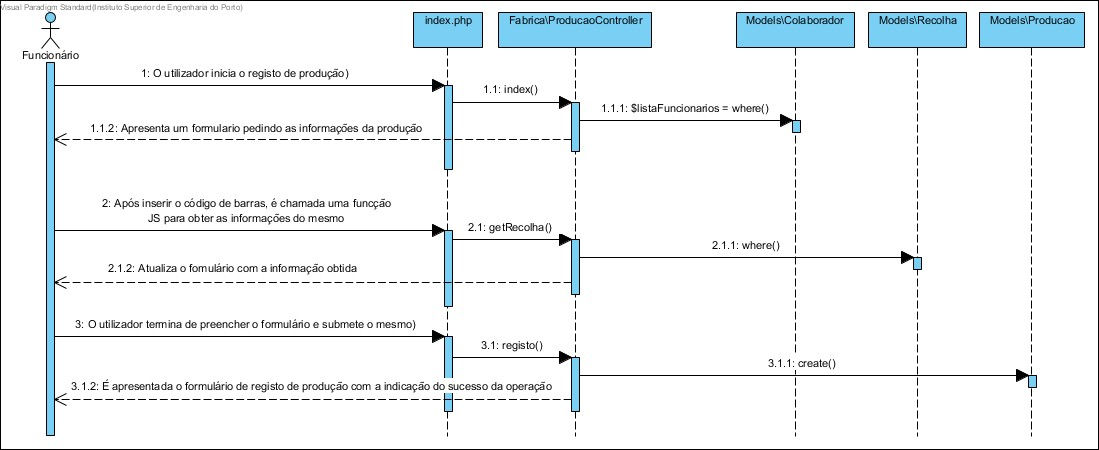
\includegraphics[width=\textwidth,keepaspectratio]{figuras/Diagramas_vp/SD_Fabrica_3_Registo_de_Produção.jpg}
%		\caption{Diagrama de Sequência registo de produção}
%		\label{fig:sd_producao} 
%	\end{center}
%\end{figure}
\todo{falta os diagramas}
\newpage
\subsection{Aplicação Fábrica: Registo de Produto Acabado}
\subsubsection*{Descrição do caso de uso}
No registo de produto acabado, espera-se que utilizador entre na página e indique o peso do produto acabado. A informação da data deve ser indicada automaticamente pelo sistema. 

\begin{figure}[H] 
	\begin{center}
		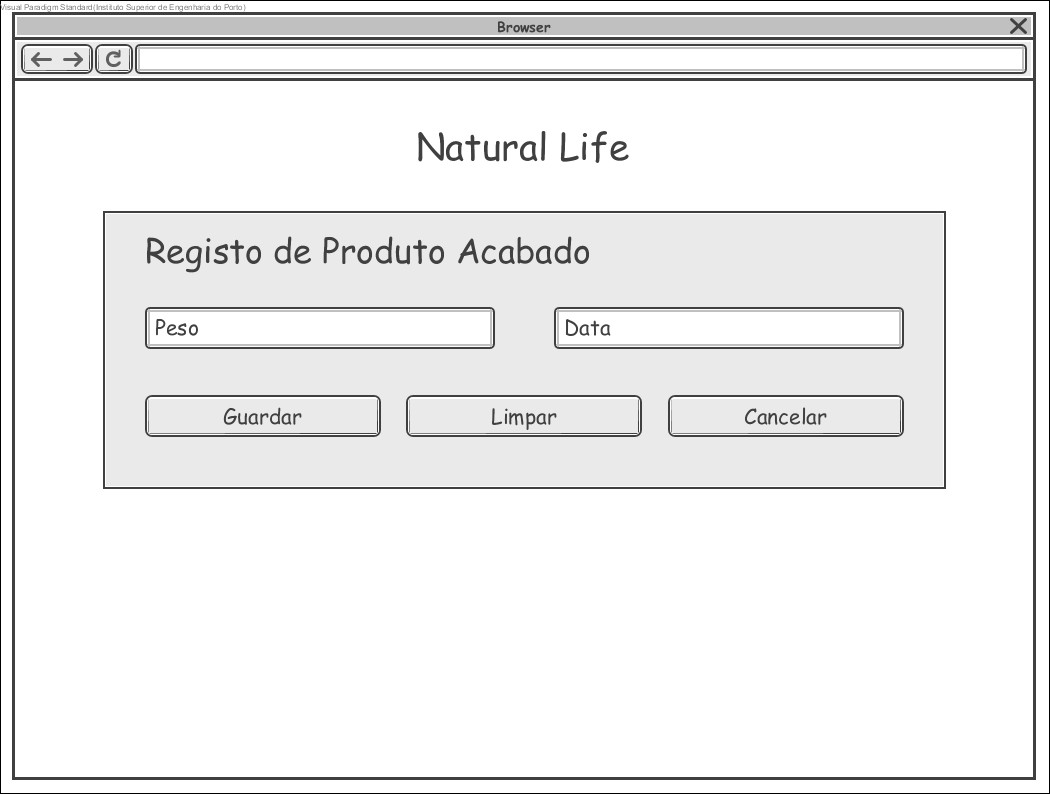
\includegraphics[width=0.60\textwidth,keepaspectratio]{figuras/Diagramas_vp/DI_Fabrica_4_Registo_de_Produto_Acabado.jpg}
		\caption{Modelo do formulário do registo de produto acabado}
		\label{fig:di_prod_acabado} 
	\end{center}
\end{figure}

\subsubsection*{Fluxo do caso de uso}
O caso de uso inicia-se com a abertura da página do registo de produto acabado. É apresentado o formulário com a data previamente preenchida. O utilizador tem de indicar o peso do produto acabado. Após indicar as informações solicitadas precisona o botão "Guardar". No final do registo é apresentada uma mensagem ao utilizador. Caso o registo seja feito com sucesso um novo separador é aberto com o código de barras para ser impresso.


\begin{figure}[H] 
	\begin{center}
		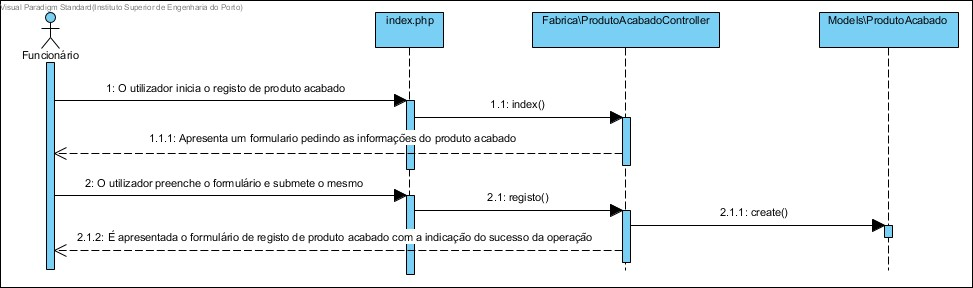
\includegraphics[width=\textwidth,keepaspectratio]{figuras/Diagramas_vp/SD_Fabrica_4_Registo_de_Produto_Acabado.jpg}
		\caption{Diagrama de sequência registo de produto acabado}
		\label{fig:sd_prod_acabado} 
	\end{center}
\end{figure}
\newpage
\subsection{Aplicação Fábrica - Registo de Saída de Produto Acabado}
\subsubsection*{Descrição do caso de uso}
No registo de produto acabado, espera-se que utilizador entre na página e indique o código de barras do produto acabado. A informação da data deve ser indicada automaticamente pelo sistema. A partir da segunda fase do projeto deverá ainda existir um campo para indicar o cliente. A aparência da \textit{view} deste caso de utilização será semelhante ao demonstrado na figura \ref{fig:di_saida_prod_acabado}. A figura  \ref{fig:di_saida_prod_acabado} (a) descreve como será a interface após concluir a primeira fase do projeto e a figura  \ref{fig:di_saida_prod_acabado} (b) descreve como será a interface após concluir a segunda. fase

\begin{figure}[H]
	\centering
	
	\begin{subfigure}[t]{0.45\linewidth}
		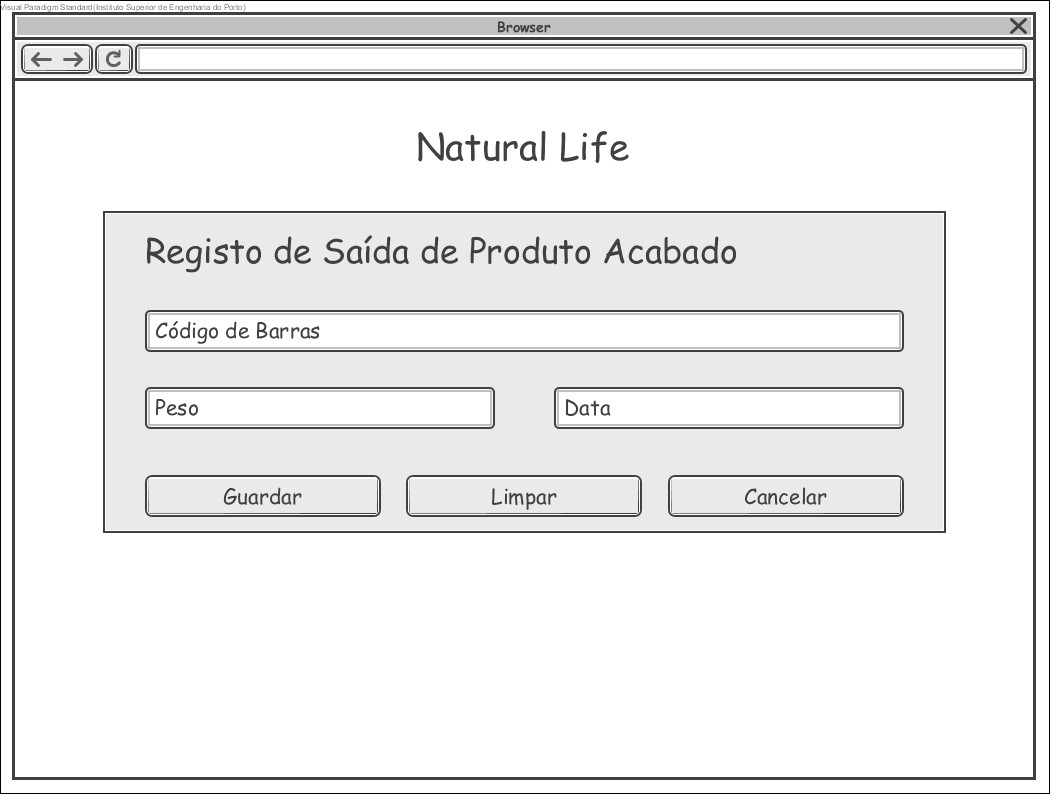
\includegraphics[width=\linewidth]{figuras/Diagramas_vp/DI_Fabrica_5_Saida_de_Produto_Acabado_1_Fase.jpg}
		\label{fig:di_saida_prod_acabado_1}
		\caption{Após concluir primeira fase}
	\end{subfigure}
	\begin{subfigure}[t]{0.45\linewidth}
		\includegraphics[width=\linewidth]{figuras/Diagramas_vp/DI_Fabrica_5_Saida_de_Produto_Acabado_2_Fase.jpg}
		\label{fig:di_saida_prod_acabado_2}
		\caption{Após concluir segunda fase}
	\end{subfigure}
	
	\caption{Modelo do menu}
	\label{fig:di_saida_prod_acabado}
\end{figure}

\subsubsection*{Fluxo do caso de utilização (2ª fase)}
O caso de uso inicia-se com a abertura da página do registo de saída de produto acabado. É apresentado o formulário com a data previamente preenchida. O utilizador tem de indicar o código de barras do produto acabado e o ID do cliente de uma lista \textit{dropdown}.  Após indicar as informações solicitadas precisona o botão "Guardar". No final do registo é apresentada uma mensagem ao utilizador. Caso o registo seja feito com sucesso um novo separador é aberto com o código de barras para ser impresso, tal como demonstrado na figura \ref{fig:sd_saida_prod_acabado}.


\begin{figure}[H] 
	\begin{center}
		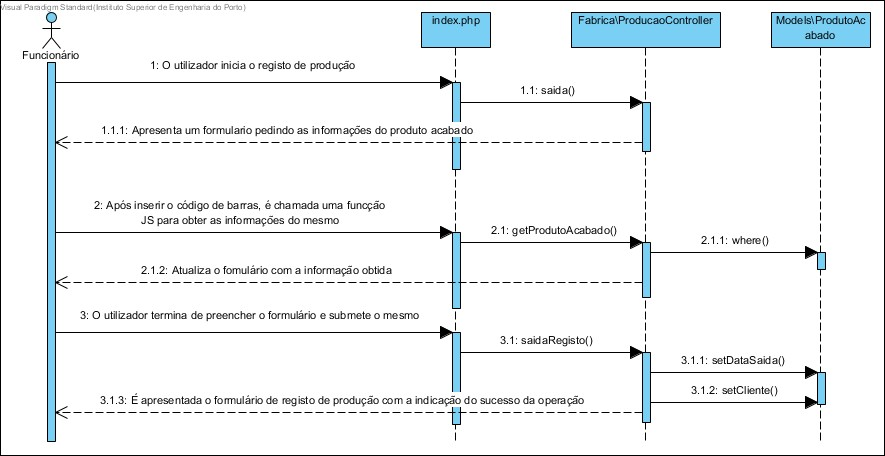
\includegraphics[width=0.95\textwidth,keepaspectratio]{figuras/Diagramas_vp/SD_Fabrica_5_Saida_de_Produto_Acabado.jpg}
		\caption{Diagrama de sequência registo de produto acabado}
		\label{fig:sd_saida_prod_acabado} 
	\end{center}
\end{figure}
\newpage
\subsection{Aplicação Fábrica: 2ª Via do código de barras}
\subsubsection*{Descrição do caso de uso}
Na obtenção de uma segunda via de um código de barras, espera-se que utilizador entre na página e indique o tipo de código de barras e o código de barras que pretende. 

\begin{figure}[H] 
	\begin{center}
		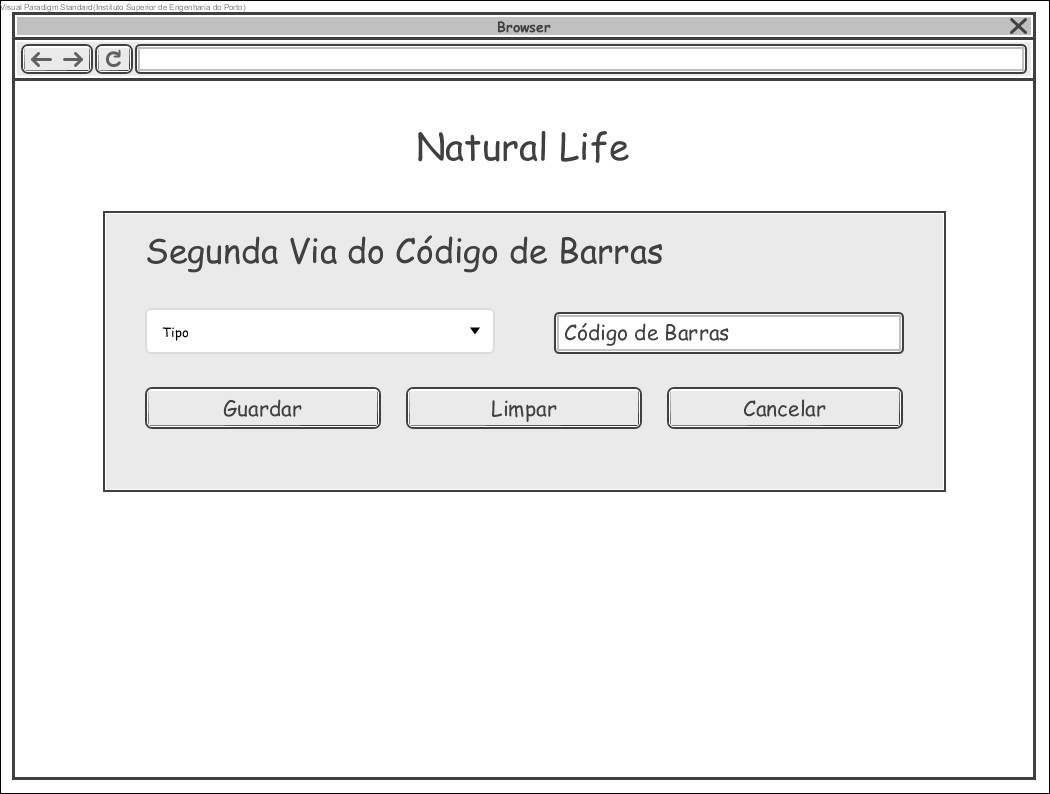
\includegraphics[width=0.60\textwidth,keepaspectratio]{figuras/Diagramas_vp/DI_Fabrica_6_2_Via_Codigo_de_Barras.jpg}
		\caption{Modelo do formulário de pedido de 2ª via de código de barras}
		\label{fig:di_2_via} 
	\end{center}
\end{figure}

\subsubsection*{Fluxo do caso de uso}
O caso de uso inicia-se com a abertura da página do pedido de segunda via de código de barras. É apresentado para o utilizador indicar o tipo de código de barras e o código de barras que pretende. Após indicar as informações solicitadas precisona o botão "Guardar". É aberto um novo separador com o código de barras solicitado para imprimir.

\todo{falta a image}
%\begin{figure}[H] 
%	\begin{center}
%		\includegraphics[width=\textwidth,keepaspectratio]{figuras/Diagramas_vp/SD_Fabrica_6_2_Via_Código_de_Barras.jpg}
%		\caption{Diagrama de sequência de pedido de 2ª via de código de barras}
%		\label{fig:sd_2_via} 
%	\end{center}
%\end{figure}
\newpage
\subsection{Aplicação Fábrica: Completar recolha}
\subsubsection*{Descrição do caso de uso}
Para completar recolha, espera-se que utilizador entre na página e indique o ID do ponto de recolha e o peso que pretende acrescentar à recolha. A informação sobre o peso total já registado bem como o histórico de incrementos será apresentado automaticamente pelo sistema. 

\begin{figure}[H] 
	\begin{center}
		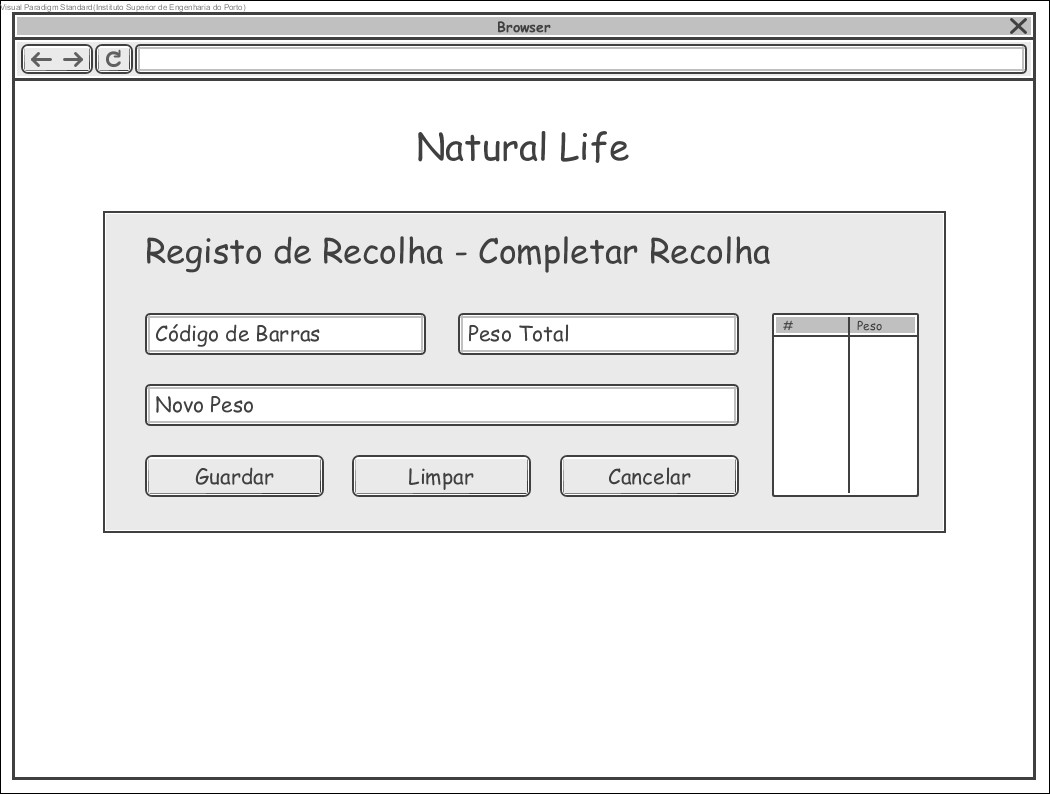
\includegraphics[width=0.60\textwidth,keepaspectratio]{figuras/Diagramas_vp/DI_Fabrica_7_Completa_Recolha.jpg}
		\caption{Modelo do formulário para incrementar o peso de uma recolha}
		\label{fig:di_completar_recolha} 
	\end{center}
\end{figure}

\subsubsection*{Fluxo do caso de uso}
O caso de uso inicia-se com a abertura da página do registo de recolha. É apresentado o formulário com a data previamente preenchida. O utilizador tem de indicar o ID do ponto de recolha numa lista de dropdown e o peso da recolha feita. Após indicar as informações solicitadas precisona o botão "Guardar". No final do registo é apresentada uma mensagem ao utilizador. Caso o registo seja feito com sucesso um novo separador é aberto com o código de barras para ser impresso.


\begin{figure}[h!] 
	\begin{center}
		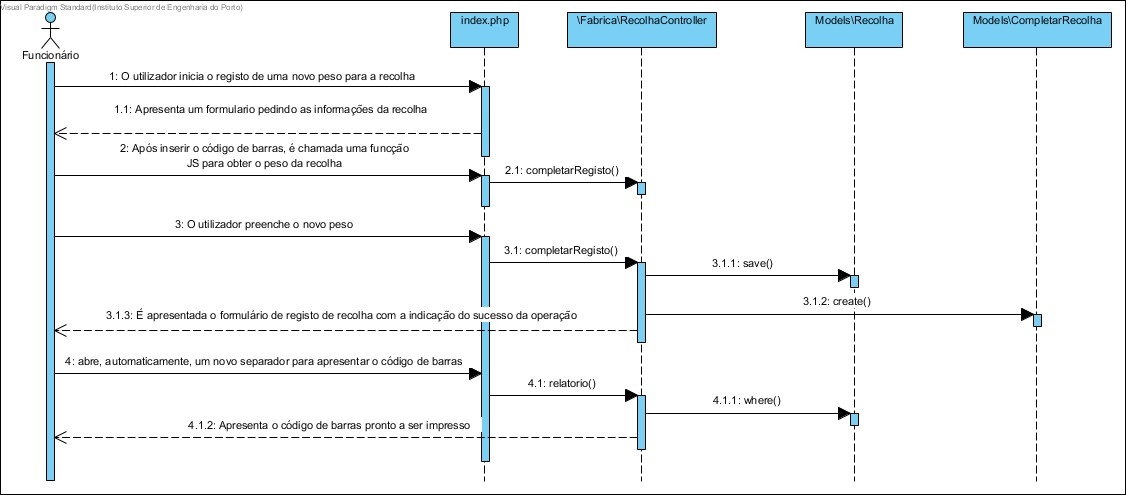
\includegraphics[width=0.90\textwidth,keepaspectratio]{figuras/Diagramas_vp/SD_Fabrica_7_Completar_Recolha.jpg}
		\caption{Diagrama de sequência para incrementar o peso de uma recolha}
		\label{fig:sd_completar_recolha} 
	\end{center}
\end{figure}
\newpage

% Aplicação Painel
\subsection{Aplicação Painel - Nota introdutória}
Os casos de uso na aplicação painel são todos iguais, independentemente do model. Desde que o caso de uso se enquadre num determinado model, os esquemas apresentados são válidos para esse model. Por esse motivo optou-se por apresentar apenas um tópico para cada caso de uso e nele é indicado os models que são compatíveis.

\subsection{Aplicação Painel - Listagem}
\subsubsection*{Descrição do caso de uso}
Para fazer uma listagem, utilizador apenas necessita de entrar na página. A aparência da \textit{view} deste caso de utilização será semelhante ao demonstrado na figura \ref{fig:di_lista}. 

\begin{figure}[H] 
	\begin{center}
		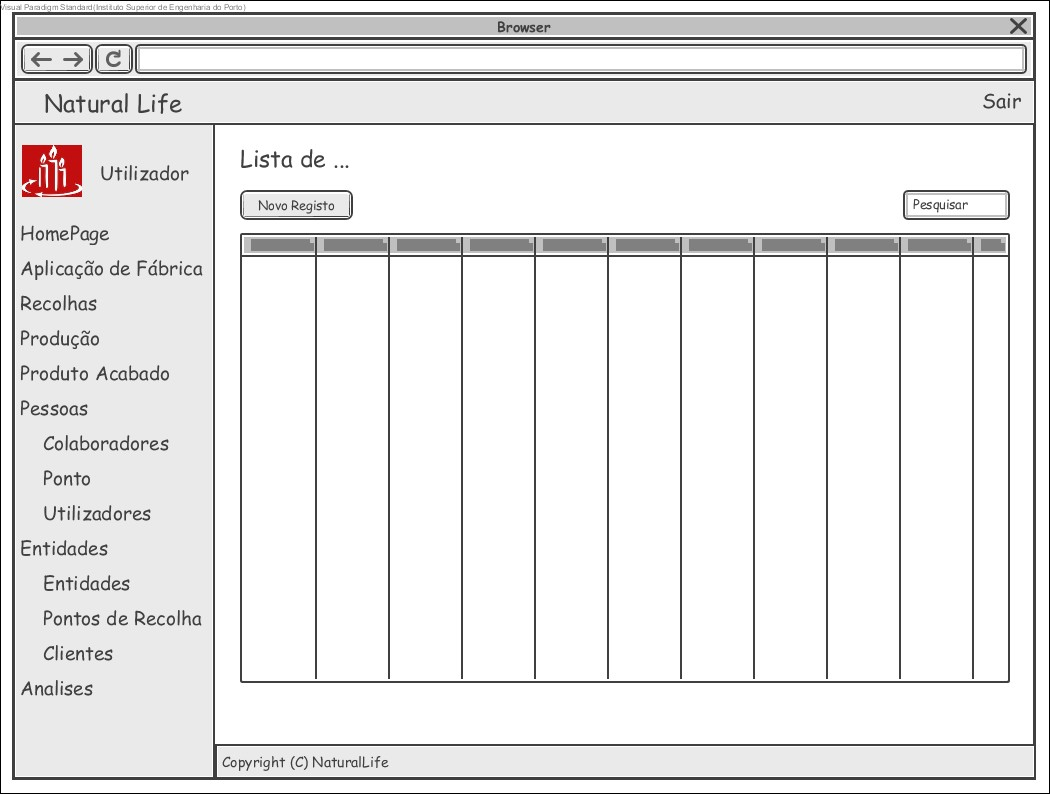
\includegraphics[width=0.60\textwidth,keepaspectratio]{figuras/Diagramas_vp/DI_Painel_1_Lista.jpg}
		\caption{Modelo da página de listagem}
		\label{fig:di_lista} 
	\end{center}
\end{figure}

\subsubsection*{Models compatíveis com o caso de uso}
Todos os models são compatíveis com este caso de uso

\subsubsection*{Fluxo do caso de utilização}
O caso de uso inicia-se com a abertura da página de listagem. É apresentado uma tabela com os dados listado e algumas opções para cada linha, tal como demonstrado na figura \ref{fig:sd_lista}.


\begin{figure}[H] 
	\begin{center}
		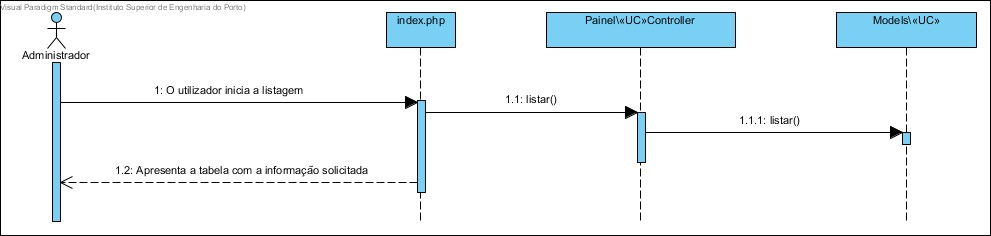
\includegraphics[width=\textwidth,keepaspectratio]{figuras/Diagramas_vp/SD_Painel_1_Listar.jpg}
		\caption{Diagrama de sequência da listagem}
		\label{fig:sd_lista} 
	\end{center}
\end{figure}
\newpage
\subsection{Aplicação Painel - Inserir}
\subsubsection*{Descrição do caso de uso}
Para inserir um registo, o utilizador necessita pressionar o botão \textit{Novo Registo}. A aparência da \textit{view} deste caso de utilização será semelhante ao demonstrado na figura \ref{fig:di_novo}. 

\begin{figure}[H] 
	\begin{center}
		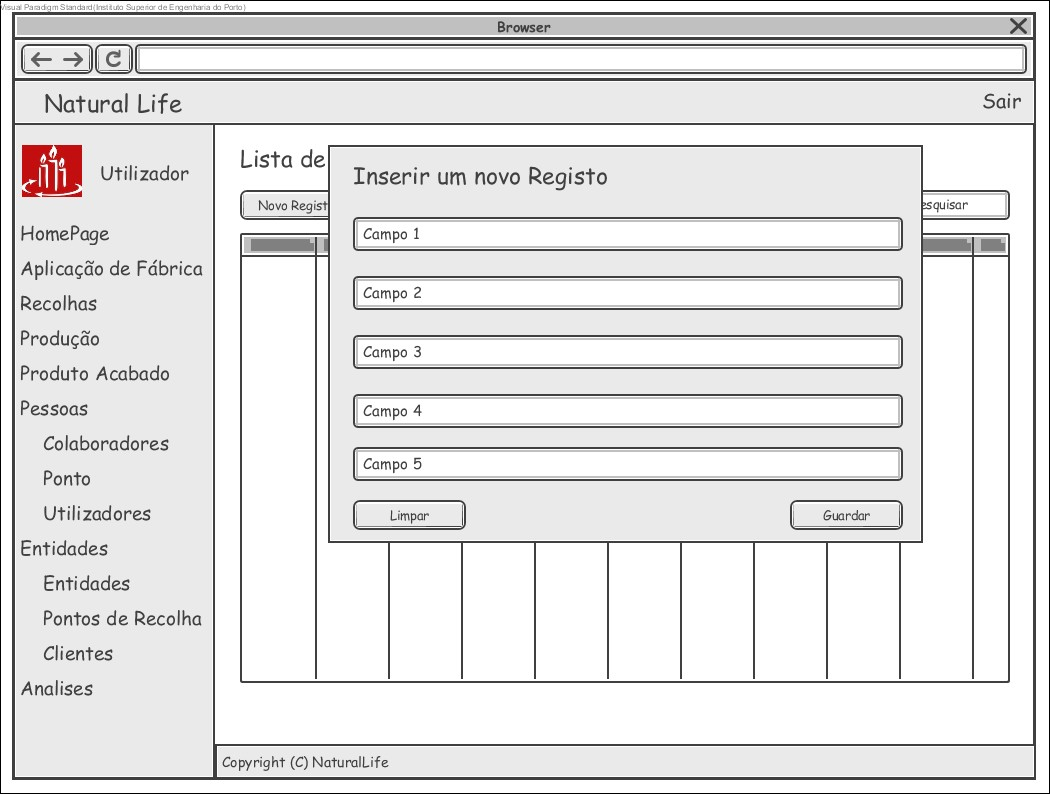
\includegraphics[width=0.60\textwidth,keepaspectratio]{figuras/Diagramas_vp/DI_Painel_2_Inserir.jpg}
		\caption{Modelo da janela de inserção na página de listagem}
		\label{fig:di_novo} 
	\end{center}
\end{figure}

\subsubsection*{\textit{Models} compatíveis com o caso de uso}
Todos os \textit{models} são compatíveis com este caso de uso

\subsubsection*{Fluxo do caso de utilização}
O caso de uso inicia-se quando o utilizador pressionar o botão novo registo na página de listagem. É apresentado uma janela flutuante com com os campos a serem preenchidos. O utilizador preenche os campos e pressiona o botão guardar. Finalizado o registo a janela fecha-se e é apresentado uma mensagem ao utilizador, tal como demonstrado na figura \ref{fig:sd_novo}.


\begin{figure}[H] 
	\begin{center}
		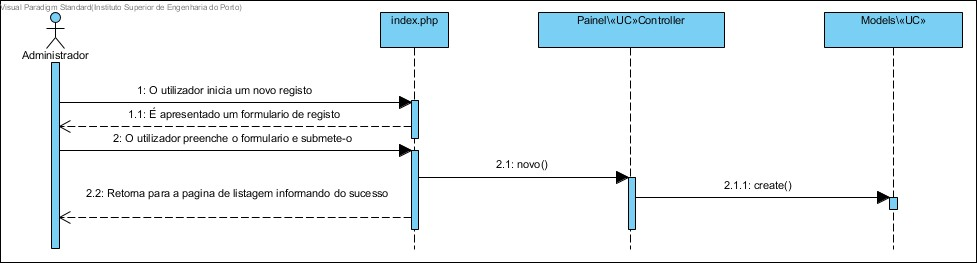
\includegraphics[width=\textwidth,keepaspectratio]{figuras/Diagramas_vp/SD_Painel_2_Inserir.jpg}
		\caption{Diagrama de sequência de inserir registo}
		\label{fig:sd_novo} 
	\end{center}
\end{figure}
\newpage
\subsection{Aplicação Painel - Editar}
\subsubsection*{Descrição do caso de uso}
Para editar um registo, o utilizador necessita pressionar o botão \textit{editar} na linha referente ao registo que pretende atualizar. A aparência da \textit{view} deste caso de utilização será semelhante ao demonstrado na figura \ref{fig:di_editar}. 

\begin{figure}[H] 
	\begin{center}
		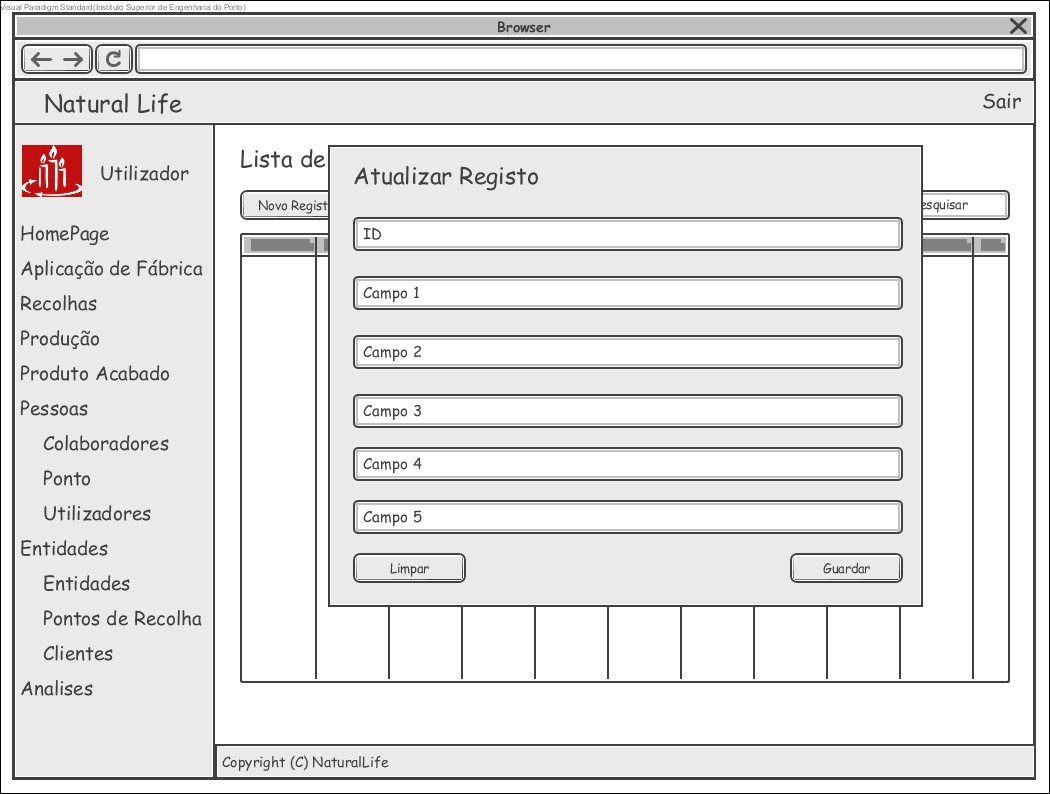
\includegraphics[width=0.60\textwidth,keepaspectratio]{figuras/Diagramas_vp/DI_Painel_3_Editar.jpg}
		\caption{Modelo da janela de edição na página de listagem}
		\label{fig:di_editar} 
	\end{center}
\end{figure}

\subsubsection*{\textit{Models} compatíveis com o caso de uso}
Este caso de uso é compatível com os \textit{models} Recolha, Produção, Produto Acabado, Colaboradores, Registo de Ponto, Entidades, Pontos de Recolha, Clientes e Analises.

\subsubsection*{Fluxo do caso de utilização}
O caso de uso inicia-se quando o utilizador pressionar o botão editar da linha do registo que pretende atualizar. O sistema vai fazer um request em background para obter as informações da base de dados e apresenta uma janela flutuante com com os campos a serem pré-preenchidos com as informações recebidas. O utilizador faz as alterações que pretende e pressiona o botão guardar. Finalizado o registo a janela fecha-se e é apresentado uma mensagem ao utilizador.


\begin{figure}[H] 
	\begin{center}
		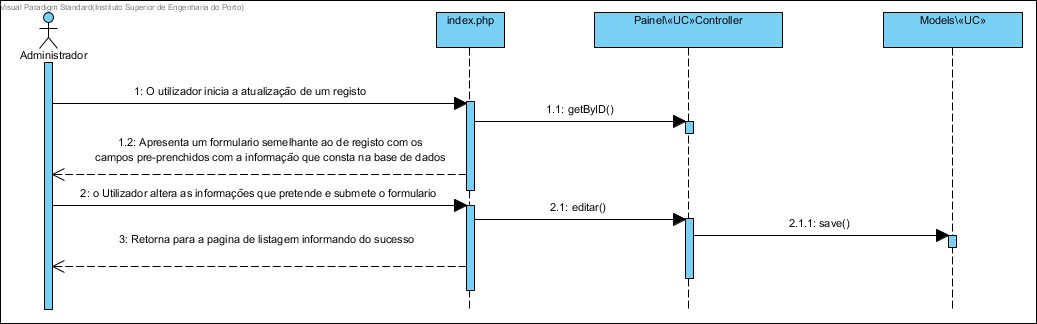
\includegraphics[width=\textwidth,keepaspectratio]{figuras/Diagramas_vp/SD_Painel_3_Editar.jpg}
		\caption{Diagrama de sequência de editar registo}
		\label{fig:sd_editar} 
	\end{center}
\end{figure}
\newpage
\subsection{Aplicação Painel: Apagar}
\subsubsection*{Descrição do caso de uso}
Para apagar um registo, o utilizador necessita pressionar o botão \textit{apagar} na linha referente ao registo que pretende atualizar. Pelo facto de ser apenas uma procedimento executado em \textit{background}, não possui nenhuma \textit{view}.

\subsubsection*{\textit{Models} compatíveis com o caso de uso}
Este caso de uso é compatível com os \textit{models} Recolha, Produção, Produto Acabado, Colaboradores, Registo de Ponto, Utilizadores, Pontos de Recolha, Clientes e Analises.

\subsubsection*{Fluxo do caso de utilização}
O caso de uso inicia-se quando o utilizador pressionar o botão apagar da linha do registo que pretende \textit{apagar}. É apresentada uma janela de confirmação. Após executar a ação é apresentada uma mensagem ao utilizador, tal como demonstrado na figura \ref{fig:sd_apagar}


\begin{figure}[H] 
	\begin{center}
		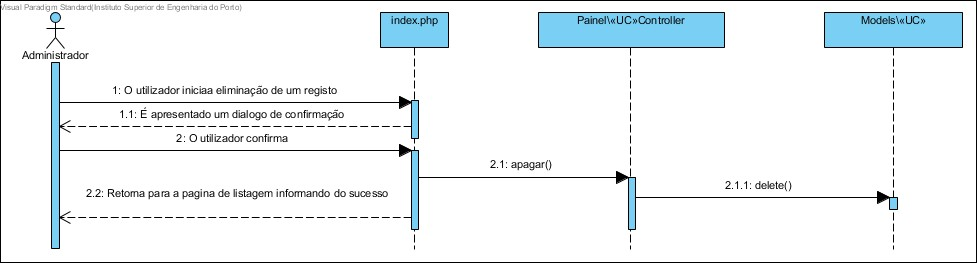
\includegraphics[width=\textwidth,keepaspectratio]{figuras/Diagramas_vp/SD_Painel_4_Apagar.jpg}
		\caption{Diagrama de sequência de apagar registo}
		\label{fig:sd_apagar} 
	\end{center}
\end{figure}
\newpage
\subsection{Aplicação Painel: Desativar/Ativar}
\subsubsection*{Descrição do caso de uso}
Desativar um registo significa que este se vai manter na base de dados, mas não irá constar mais nas UI da aplicação de Fábrica. Para \textit{desativar/ativar} um registo, o utilizador necessita pressionar o botão \textit{desativar/ativar} na linha referente ao registo que pretende atualizar. Pelo facto de ser apenas uma procedimento executado em \textit{background}, não possui nenhuma view.

\subsubsection*{\textit{Models} compatíveis com o caso de uso}
Este caso de uso é compatível com os \textit{models} Colaboradores, Pontos de Recolha e Clientes.

\subsubsection*{Fluxo do caso de utilização}
O caso de uso inicia-se quando o utilizador pressionar o botão desativar/ativar da linha do registo que pretende desativar/ativar. Após executar a ação é apresentada uma mensagem ao utilizador, tal como demonstrado na figura \ref{fig:sd_desativar}


\begin{figure}[H] 
	\begin{center}
		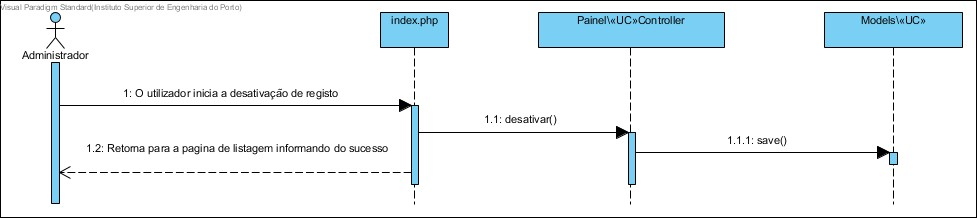
\includegraphics[width=\textwidth,keepaspectratio]{figuras/Diagramas_vp/SD_Painel_5_Desativar.jpg}
		\caption{Diagrama de sequência de desativar/ativar registo}
		\label{fig:sd_desativar} 
	\end{center}
\end{figure}
\newpage
\subsection{Aplicação Painel - segunda via código de barras}
\subsubsection*{Descrição do caso de uso}
Caso pretenda, um utilizador do painel também pode re-imprimir um código de barras sem necessidade de abrir a aplicação Fábrica. Para isso o utilizador necessita pressionar o botão\textit{ segunda via} da linha referente ao registo que pretende atualizar. Pelo facto de ser apenas uma procedimento executado em \textit{background}, não possui nenhuma \textit{view}.

\subsubsection*{\textit{Models} compatíveis com o caso de uso}
Este caso de uso é compatível com os \textit{models} Recolhas, Produto Acabado.

\subsubsection*{Fluxo do caso de utilização}
O caso de uso inicia-se quando o utilizador pressionar o botão 2ª via de código de barras da linha do registo. Um novo separador abre-se com o código de barras pronto a ser impresso, tal como demonstrado na figura \ref{fig:sd_2_via_painel}.


\begin{figure}[H] 
	\begin{center}
		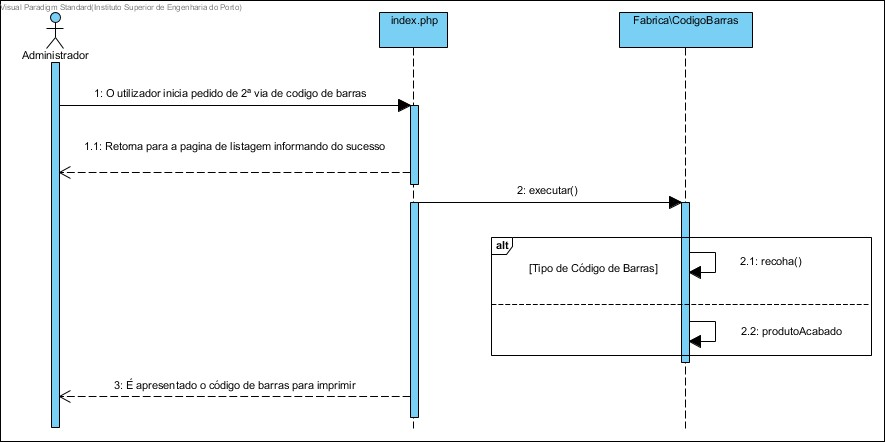
\includegraphics[width=\textwidth,keepaspectratio]{figuras/Diagramas_vp/SD_Painel_6_2_via_Codigo_de_Barras.jpg}
		\caption{Diagrama de sequência imprimir 2ª via do código de barras}
		\label{fig:sd_2_via_painel} 
	\end{center}
\end{figure}
\newpage
\subsection{Aplicação Fábrica: Executar Analise}
\subsubsection*{Descrição do caso de uso}
Uma analise é um script SQL com uma query personalizada. Para executar uma analise basta pressionar o botão executar na linha referente à analise pretendida.

\subsubsection*{Models compatíveis com o caso de uso}
Este caso de uso é apenas compatível com o model Analises.

\subsubsection*{Fluxo do caso de uso}
O caso de uso inicia-se quando o utilizador pressionar o botão executar da linha do registo que pretende executar. A página vai recarregar, fazendo aparacer o resultado da analise pedida.


\begin{figure}[H] 
	\begin{center}
		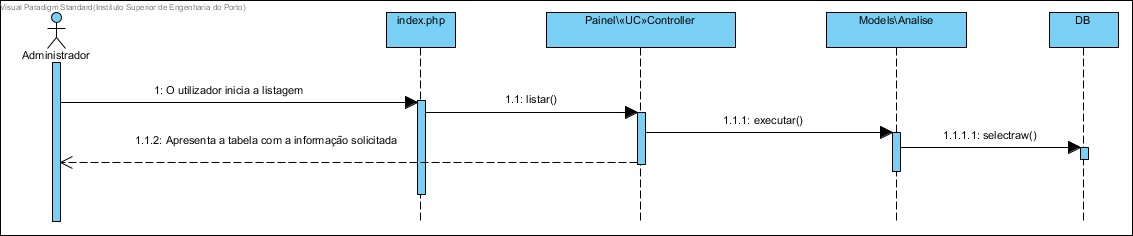
\includegraphics[width=\textwidth,keepaspectratio]{figuras/Diagramas_vp/SD_Painel_7_Executar_Analise.jpg}
		\caption{Diagrama de sequência para executar uma recolha}
		\label{fig:sd_executar analise} 
	\end{center}
\end{figure}
\newpage

\section{Script de verificação da integridade de informação}
Concluído a projeção de cada caso de uso, é necessario planear o ultimo componente do sistema, os scripts responsáveis por emitir alertas quando existem dados não coerentes nas tabelas da base de dados. Segundo a lista de requisitos são três os scripts a serem desenvolvidos: Pontos de Recolha, Registos de Ponto e Produção.

\subsection{Principio de funcionamento}
Pretende-se que todos os scripts funcionem de um modo igual: uma SQL stored procedure no Microsft SQL Server que é executada todos os dias. Essa stored procedure contem um query especifico que visa identificar as situações que necessitam ser analisadas. Essa query é executada e caso haja retorno é enviado um email com essa informação (figura \ref{fig:stored_procedure})

\begin{figure}[h] 
	\begin{center}
		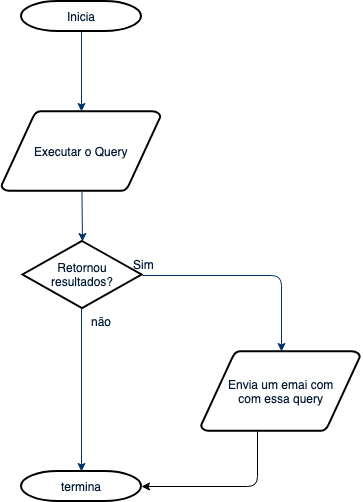
\includegraphics[width=0.30\textwidth,keepaspectratio]{figuras/FluxogramaEmail.png}
		\caption{Fluxograma das stored procedures}
		\label{fig:stored_procedure} 
	\end{center}
\end{figure}


\subsection{Objetivo de execução}
Cada uma das uma das stored procedures será criada para identificar determinados padrões e reportar-los via email.\\
A stored procedure Pontos de Recolha serve para identificar Pontos de Recolha cujo o fim de protocolo esta-se a aproximar.
A stored procedure Registos de Ponto serve para identificar registos de ponto que estão em falta ou duplicados
A stored procedure Produção serve para identificar as produções cujo o somatório dos peso é superior ao peso da recolha. 